% Requires \usepackage{graphicx}. Use figure instead of figure* for a
% single-column layout; the vector PDF will scale without quality loss.
\begin{figure*}[t]
  \centering
  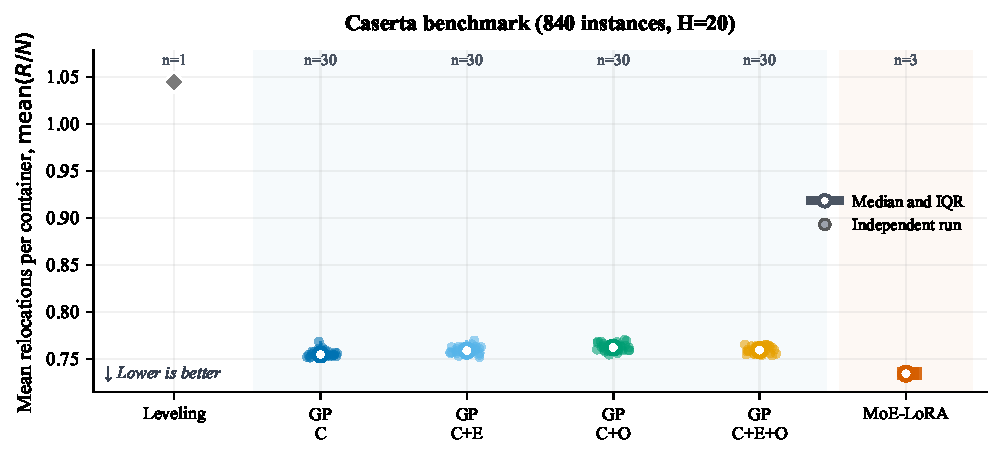
\includegraphics[width=\textwidth]{figures/fig_gp_moe_leveling_h20.pdf}
  \caption{Distribution of H=20 performance on the 840-instance Caserta
  benchmark. Points denote independent runs; open circles and thick vertical
  segments show the median and interquartile range, respectively, while thin
  segments show the minimum--maximum range. GP uses 30 independently evolved
  rules per terminal set, MoE-LoRA uses three formal seeds, and Leveling is
  deterministic and horizon-independent. Lower is better; no seed was selected
  using Caserta performance.}
  \label{fig:gp_moe_leveling_h20}
\end{figure*}
